\subsubsection{The diodes bridge example}

\begin{figure}[h]
\centerline{
 \scalebox{0.7}{
    \input{../ace/Bridge.pstex_t}
 }
}
 \caption{Diodes bridge}
\label{fig-Diode-bridge}
\end{figure}





\paragraph{The Diode non smooth model instance} without any offset (\ref{eq:63}) is reminded :
\[ y = -U_{ns}\]
\[ I_{ns} = l \]
\[0 \leq y \, \perp \, l \geq 0\]


\paragraph{Global formulation}, it consists in assembling the 4 diodes in a matrix formulation.

\[ \lambda =(l_{1},l_{2},l_{3},l_{4})\]
\[Z_{ns}=0X+0Z_{s}+Id\lambda\]
\[Y=\left(\begin{array}{cc}
0&0\\
0&0\\
0&0\\
0&0\end{array}\right) x+
\left(\begin{array}{ccc}
0&1&0\\
0&0&1\\
1&0&-1\\
1&-1&0\end{array}
\right) Z_{s} + 0Z_{ns} +0\lambda\]

\[0 \leq Y \, \perp \, \lambda \geq 0\]

Note that :
\begin{itemize}

  \item[--] The diode 2 is managed by the couple $(l_1,y_1)$
  \item[--] The diode 3 is managed by the couple $(l_2,y_2)$
  \item[--] The diode 4 is managed by the couple $(l_3,y_3)$
  \item[--] The diode 5 is managed by the couple $(l_4,y_4)$
\end{itemize}
\paragraph{Unknowns} must be chosen before write the circuit equations

x = $^{t}(U_{1},I_{7})$,
$Z_{ns}=^{t}(I_{2},I_{3},I_{4},I_{5}$),
$z = ^{t}(V_{1},V_{2},V_{3})$
\paragraph{Matrices formulation}, in this paragraph, the physicals laws are written with
complementarity constraints. The system obtained is named a Mixed Linear Complementarity System.
\[
\left(\begin{array}{c}
  
x'=\left(\begin{array}{cc}
0 &\frac{-1}{C}\\
0&0\end{array} \right)x
+\left(\begin{array}{ccc}
0&0&0\\
\frac{1}{L}&0&0\end{array} \right)z
+\left(\begin{array}{cccc}
0&0&\frac{1}{C}&\frac{-1}{C}\\
0&0&0&0\end{array} \right)Z_{ns}
\\
0=\left(\begin{array}{cc}
0 &0\\
0 &0\\
1 &0\end{array} \right)x
+\left(\begin{array}{ccc}
0&\frac{1}{R}&\frac{-1}{R}\\
0&\frac{-1}{R}&\frac{1}{R}\\
0&1&0\end{array} \right)z
+\left(\begin{array}{cccc}
1&0&0&1\\
0&+1&1&0\\
0&0&0&0\end{array} \right)Z_{ns}
\\
Z_{ns}=Dx+0z+Id\lambda\\
Y=0x+
\left(\begin{array}{ccc}
0&1&0\\
0&0&1\\
1&0&-1\\
1&-1&0\end{array}
\right) z + 0Z_{ns} +0\lambda\\

0 \leq Y \, \perp \, \lambda \geq 0

\end{array}
\right)
\]
The physical laws written in the previous system are :
\begin{itemize}
\item[--] The first is the Kirchhoff Current Law  at the node 1.
\item[--] The second line is the constitutive inductor law.
\item[--] The third line is the Kirchhoff Current Law at the node 3.
\item[--] The fourth line is the Kirchhoff Current Law at node 2.
\item[--] The fifth line is $U_1 + V_1=0$.
\end{itemize}


\paragraph{Simulation}, The Mixed Linear Complementarity System is discretized, it leads to a Mixed
Complementarity Problem solved at each time step. See Following
section for more details about the discretization. \\
C= 1 uF\\
L= 10 mH\\
R= 1000 $\Omega$\\
The simulation computed 450 steps with a $10^{-6}s$ fixed time step. The figure
\ref{fig-Diode-sim} shows the tension in the resistor branch.


\begin {figure}[h]
%GNUPLOT: LaTeX picture with Postscript
\begin{picture}(0,0)%
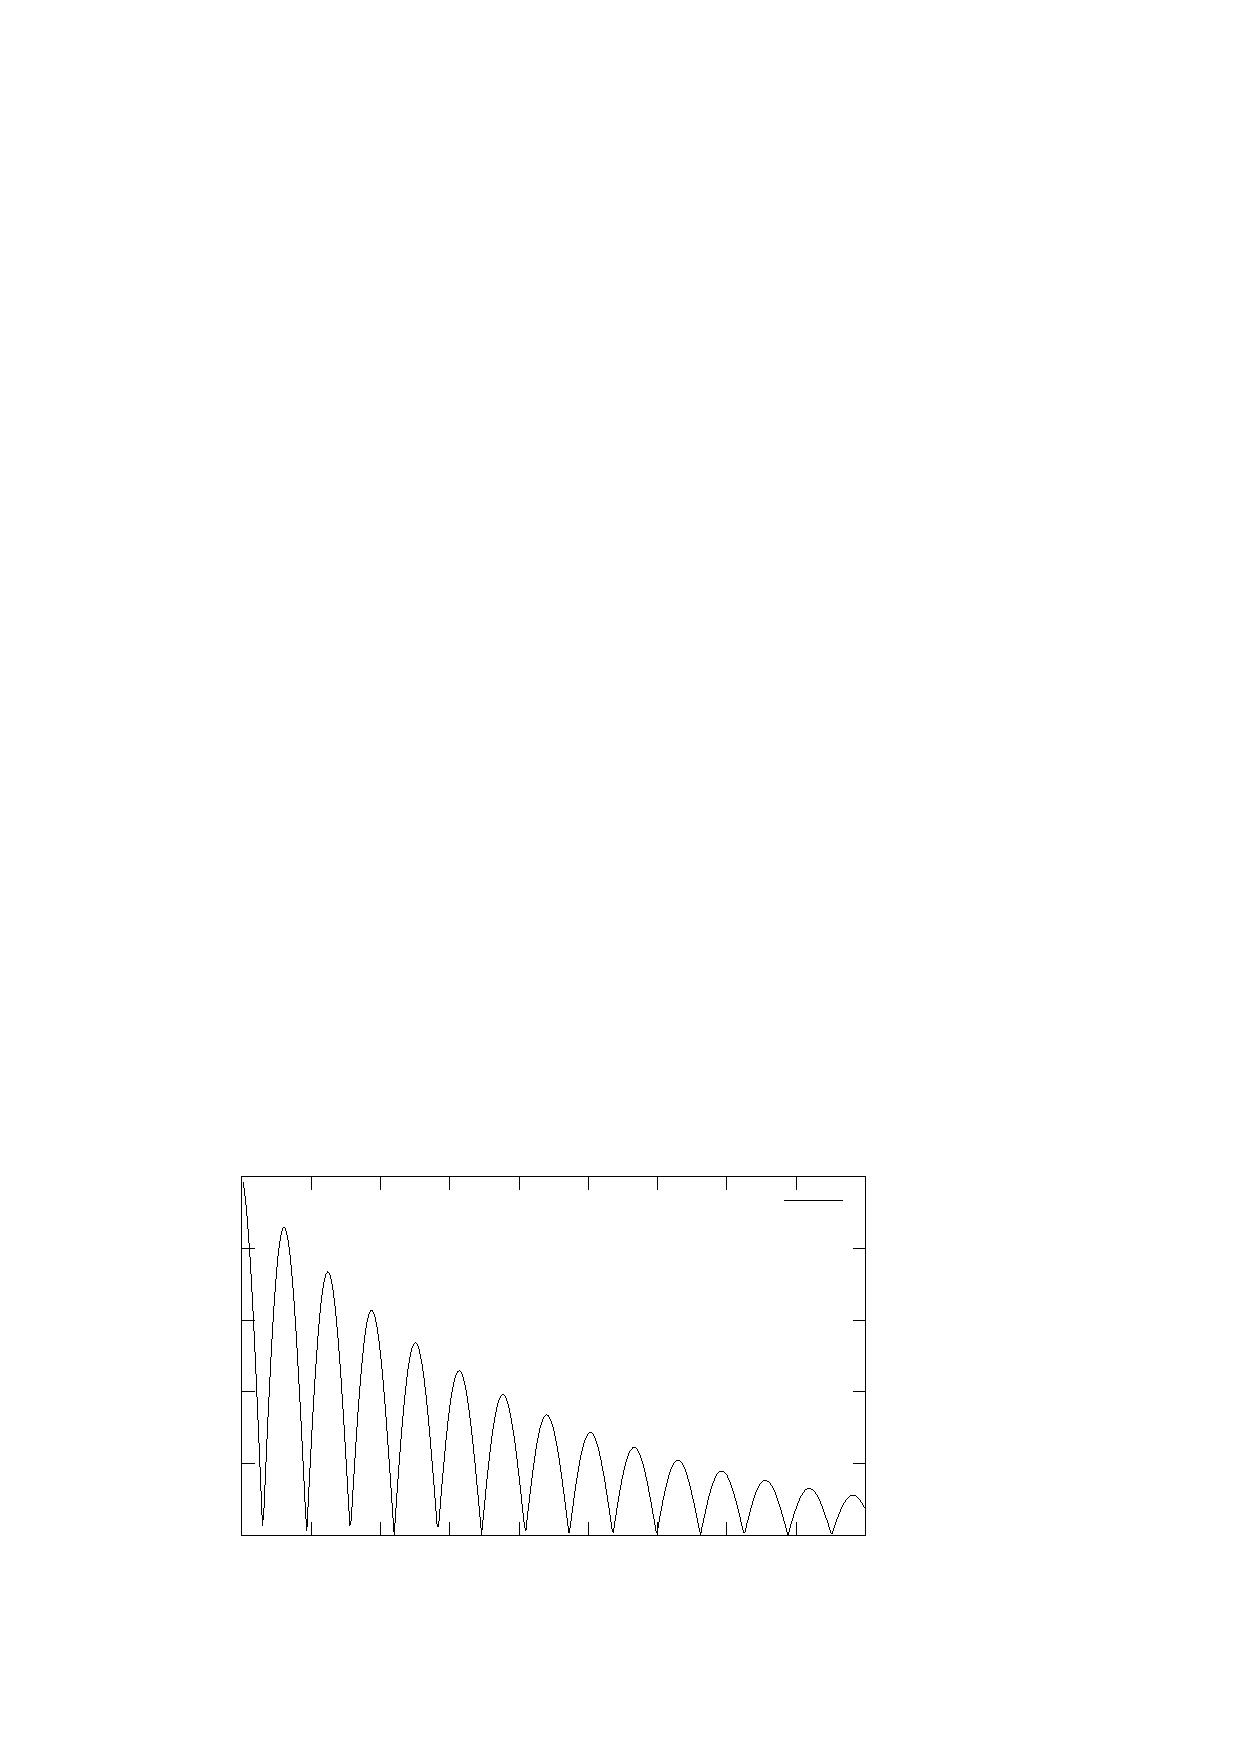
\includegraphics{diodes}%
\end{picture}%
\begingroup
\setlength{\unitlength}{0.0200bp}%
\begin{picture}(18000,10800)(0,0)%
\put(1925,1650){\makebox(0,0)[r]{\strut{} 0}}%
\put(1925,3370){\makebox(0,0)[r]{\strut{} 2}}%
\put(1925,5090){\makebox(0,0)[r]{\strut{} 4}}%
\put(1925,6810){\makebox(0,0)[r]{\strut{} 6}}%
\put(1925,8530){\makebox(0,0)[r]{\strut{} 8}}%
\put(1925,10250){\makebox(0,0)[r]{\strut{} 10}}%
\put(2200,1100){\makebox(0,0){\strut{} 0}}%
\put(3864,1100){\makebox(0,0){\strut{} 50}}%
\put(5528,1100){\makebox(0,0){\strut{} 100}}%
\put(7192,1100){\makebox(0,0){\strut{} 150}}%
\put(8856,1100){\makebox(0,0){\strut{} 200}}%
\put(10519,1100){\makebox(0,0){\strut{} 250}}%
\put(12183,1100){\makebox(0,0){\strut{} 300}}%
\put(13847,1100){\makebox(0,0){\strut{} 350}}%
\put(15511,1100){\makebox(0,0){\strut{} 400}}%
\put(17175,1100){\makebox(0,0){\strut{} 450}}%
\put(550,5950){\rotatebox{90}{\makebox(0,0){\strut{}U23}}}%
\put(9687,275){\makebox(0,0){\strut{}time e-5 s}}%
\put(14950,9675){\makebox(0,0)[r]{\strut{}'DiodeBridge.traj'}}%
\end{picture}%
\endgroup
\endinput

\caption{Diode bridges simulation}
\label{fig-Diode-sim}
\end {figure} 
